% !TeX encoding = UTF-8
% !TeX program = xelatex

%%+++++++++++++++++++++++++++++++++++++++++++++++++++++++++
%%        专业型学位, 人文社科大类章节编号用中文,
%%+++++++++++++++++++++++++++++++++++++++++++++++++++++++++
%\documentclass[profesdegree,chinesetitlenum]{hainnuthesis}

%%+++++++++++++++++++++++++++++++++++++++++++++++++++++++++
%%        专业型学位, 理工科大类章节编号用数字,
%%+++++++++++++++++++++++++++++++++++++++++++++++++++++++++
%\documentclass[profesdegree,arabictitlenum]{hainnuthesis}

%%+++++++++++++++++++++++++++++++++++++++++++++++++++++++++
%%        学术型学位, 人文社科大类章节编号用中文,
%%+++++++++++++++++++++++++++++++++++++++++++++++++++++++++
%\documentclass[academdegree,chinesetitlenum]{hainnuthesis}

%%+++++++++++++++++++++++++++++++++++++++++++++++++++++++++
%%        学术型学位, 理工科大类章节编号用数字,
%%+++++++++++++++++++++++++++++++++++++++++++++++++++++++++
\documentclass[academdegree,arabictitlenum]{hainnuthesis}

%% 随机文本(测试使用)
\usepackage{lipsum,zhlipsum}

%% 超链接设定
\usepackage[colorlinks,
			linkcolor=black,
			anchorcolor=blue,
			citecolor=blue]{hyperref}


%%你可以在下面的文件中添加自己常用的宏定义,简化命令的使用
\usepackage{xcolor}
\newcommand{\blue}[1]{\textcolor{blue}{#1}}
\newcommand{\green}[1]{\textcolor{green}{#1}}
\newcommand{\red}[1]{\textcolor{red}{#1}}
\newcommand{\cyan}[1]{\textcolor{cyan}{#1}}
\newcommand{\magenta}[1]{\textcolor{magenta}{#1}}
\newcommand{\yellow}[1]{\textcolor{yellow}{#1}}

\renewcommand{\tablename}{表}
\renewcommand{\figurename}{图}
\renewcommand{\lstlistingname}{代码}

\newtheorem{definition}{{\heiti\hspace*{2em}定义}}[chapter]
\newtheorem{theorem}{{\heiti\hspace*{2em}定理}}[chapter]
\newtheorem{lemma}{{\heiti\hspace*{2em}引理}}[chapter]
\newtheorem{proposition}{{\heiti\hspace*{2em}命题}}[chapter]
\newtheorem{example}{{\heiti\hspace*{2em}例}}[chapter]
\newtheorem{corollary}{{\heiti\hspace*{2em}推论}}[chapter]
\newtheorem{property}{{\heiti\hspace*{2em}性质}}[chapter]

\newcommand{\Analysis}{\textbf{分析:}~}
\newcommand{\RightSolution}{\textbf{正解:}~}
\newcommand{\ErrorSolution}{\textbf{错解:}~}




%
%数学公式写作定义
%------------------------------------------------------------
%    MathDef.tex   你可以修改或设定自己的数学公式环境定义
%------------------------------------------------------------

\usepackage[electronic]{ifsym}
\usepackage{indentfirst}
\usepackage{latexsym}

%%\usepackage{unicode-math}
%\usepackage{mathpazo}
%%\usepackage[mathpazo]{flexisym}
\usepackage{bm}
\usepackage{bbm}
\usepackage{mathrsfs}

\usepackage{amsmath}
%\usepackage{amssymb}
\usepackage{amsfonts}
%\usepackage{amsthm}
\usepackage{amscd}
\usepackage{pifont}
%\usepackage{wasysym}
\usepackage[mathscr]{euscript}

\usepackage[all]{xy}  % 画交换图


\newcommand{\op}[1]{\mathcal{#1}}
\newcommand{\Real}{\mathbb{R}}
\newcommand{\Complex}{\mathbb{C}}
\newcommand{\Proj}{\mathbb{P}}
\newcommand{\field}[1]{\mathbb{#1}}
\newcommand{\cc}[1]{\overline{#1}}   % complex congugate
\newcommand{\hc}[1]{{#1}^{\dagger}}  % Hermitian congugate

%%%%%%%%%%%%%%%%%%%%%%%%%%%%%%%%%
%%   Operators
%%%%%%%%%%%%%%%%%%%%%%%%%%%%%%%%%
\DeclareMathOperator{\Ker}{\mathrm{Ker}}
\DeclareMathOperator{\Image}{\mathrm{Im}}
\DeclareMathOperator{\argmin}{\mathrm{argmin}}
\DeclareMathOperator{\SSE}{\mathrm{SSE}}
\DeclareMathOperator{\dist}{\mathrm{dist}}
\DeclareMathOperator*{\union}{\cup}
\DeclareMathOperator{\polydeg}{\mathrm{deg}}
\DeclareMathOperator{\lspan}{\mathrm{span}}
\DeclareMathOperator{\diag}{\mathrm{diag}}
\DeclareMathOperator{\rank}{\mathrm{rank}}
\DeclareMathOperator{\trace}{\mathrm{tr}}
\DeclareMathOperator{\Dim}{\mathrm{dim}}
\DeclareMathOperator{\Dom}{\mathrm{Dom}}
\DeclareMathOperator{\Range}{\mathrm{Range}}
\DeclareMathOperator{\Null}{\mathrm{Null}}
\DeclareMathOperator{\FFT}{\mathrm{FFT}}
\DeclareMathOperator{\DFT}{\mathrm{DFT}}    % Discrete Fourier Transformation
\DeclareMathOperator{\id}{\mathbbm{1}}
\DeclareMathOperator{\dif}{\mathrm{d}}
\DeclareMathOperator{\Hom}{\mathrm{Hom}}
\DeclareMathOperator{\sign}{\mathrm{sign}}
\DeclareMathOperator{\Ann}{\mathrm{Ann}}
\DeclareMathOperator{\dB}{\mathrm{dB}}
\DeclareMathOperator{\GF}{\mathbb{GF}} % Galois Filed
\DeclareMathOperator{\sinc}{\mathrm{sinc}}      % sin count function, sinc(x) = sin (\pi x)/(\pi x)
\DeclareMathOperator{\rect}{\mathrm{rect}}      % regutangular impulse
\DeclareMathOperator{\erf}{\mathrm{erf}}
\DeclareMathOperator{\erfc}{\mathrm{erfc}}
\DeclareMathOperator{\Q}{\mathrm{Q}}
\DeclareMathOperator{\const}{\mathrm{const}}

\DeclareMathOperator{\vecs}{\mathrm{vecs}}
\DeclareMathOperator{\Zern}{\mathrm{Z}}
\DeclareMathOperator{\grad}{\overrightarrow{\mathrm{grad}}}
\DeclareMathOperator{\dive}{\mathrm{div}}
\DeclareMathOperator{\curl}{\overrightarrow{\mathrm{rot}}}

\newcommand{\atan}{\mathrm{atan2}}

\newcommand{\mapstset}[2]{\left.{#1}\right|_{#2}}


%%%%%%%%%%%%%%%%%%%%%%%%%%%%%%%%%%%%%%%%%%%%%%%%%%%%%%%%%%%%%%%
%  CV notations
%%%%%%%%%%%%%%%%%%%%%%%%%%%%%%%%%%%%%%%%%%%%%%%%%%%%%%%%%%%%%%%
\newcommand{\univset}[1]{\mathscr{#1}} % universal set
\newcommand{\setclass}[1]{\mathcal{#1}} % set class
\newcommand{\manifold}[1]{\mathcal{#1}}
\newcommand{\chart}[1]{\mathscr{#1}}  % coordinate chart in manifold
\newcommand{\manpt}[1]{\mathrm{#1}}     % point in a manifold
\newcommand{\vecfield}{\mathscr{X}}
\newcommand{\TpM}[2]{\mathscr{T}_{#1}(#2)}
\newcommand{\cTpM}[2]{\mathscr{T}^*_{#1}(#2)}
\newcommand{\tanspace}[1]{\mathscr{T}(#1)}          % tangent space
\newcommand{\cotspace}[1]{\mathscr{T}^*(#1)}       % cotangent space
\newcommand{\tanbundle}[1]{\mpair{#1}{\mathscr{T}(#1)}} % tangent fibre bundle
\newcommand{\ctanbundle}[1]{\mpair{#1}{\mathscr{T}^*(#1)}} % cotangent fibre bundle
\newcommand{\Diff}{\mathrm{Diff}} % diffeomorphism

\newcommand{\img}[1]{\mathcal{#1}}      % image frame variable
\newcommand{\wopt}[1]{\bf{#1}}          % world point  4-vector
\newcommand{\impt}[1]{\bf{#1}}          % image广。矩阵求导与微分,是计算机视觉、信号处理以及其他很多工程领域都有着广泛的应用。 point  3-vector
\newcommand{\imli}[1]{\bf{#1}}          % image line   3-vector
\newcommand{\cam}[1]{\bf{#1}}       % camera projection 3-by-4 matrix
\newcommand{\IAC}[1]{\tinv{#1}\inv{#1}}
\newcommand{\conic}[1]{\mathcal{#1}}    % conics
\DeclareMathOperator{\MOSAIC}{MOSAIC}  % 全景拼接
\DeclareMathOperator{\GetStrip}{GetStrip} % 图像条带选取
\newcommand{\strip}[1]{\overline{#1}} % image strip
\DeclareMathOperator*{\mosaic}{\sqcup}
\newcommand{\woptl}[1]{\scrut{\mathbf{#1}}{loc}}   %local frame, world coordinate point  4-vector
\newcommand{\woptg}[1]{\scrut{\mathbf{#1}}{glb}}   %global frame, world coordinate point  4-vector
\newcommand{\woptsl}[1]{\scrut{\mathfrak{#1}}{loc}}   %local frame, world coordinate point  4-vector
\newcommand{\woptsg}[1]{\scrut{\mathfrak{#1}}{glb}}   %global frame, world coordinate point  4-vector
\newcommand{\imsz}[2]{\texttt{#1} \times \texttt{#2}}  % image size




\DeclareMathOperator{\Int}{\mathrm{int}} % interior of a set
\DeclareMathOperator{\Ext}{\mathrm{ext}} % exterior of a set
\DeclareMathOperator{\bry}{\partial} % boundary operator

\newcommand{\gso}{\mathrm{g^2o}}

 
\DeclareMathOperator{\mtv}{\mathrm{vec}}    % 矩阵按列堆栈生成向量
\DeclareMathOperator{\smtv}{\mathrm{vecs}}  % 对称矩阵按行生成向量
\newcommand{\vtm}[1]{\inv{\mtv}(#1)}        % 向量整形生成矩阵
\newcommand{\vtsm}[1]{\inv{\smtv}(#1)}      % 向量按行生成对称矩阵
\newcommand{\oplift}[1]{{#1}^\wedge}   % 三维向量提升为三阶反对称矩阵
\newcommand{\opdown}[1]{{#1}^\lor}     % 三阶反对称矩阵降格为三维向量 
\newcommand{\vtam}[1]{\scrdm{\left[#1\right]}{\times}}      % 三维向量整形为三阶反对称矩阵

\newcommand{\liebraket}[2]{\left[#1, #2\right]} % Lie括号

%\DeclareMathOperator{\vecm}{vec}                     % 按列向量堆栈(一般矩阵)
%\DeclareMathOperator{\unvm}{unvec}
%\DeclareMathOperator{\vecs}{vecs} 
%\newcommand{\vecmat}[1]{\vecm{\left( {#1} \right)}}
%\newcommand{\vecsmat}[1]{\vecs{\left( {#1} \right)}}
%\newcommand{\vecasym}[1]{[#1]_\times}   % antisymmetric matrix from a vector
%\newcommand{\matTOvec}[1]{\vecm{\left( #1 \right)}}
%\newcommand{\smatTOvec}[1]{\vecs{\left( #1 \right)}}
%\newcommand{\vecTOasym}[1]{[#1]_{_\times}}

%\newcommand{\matTOvec}[1]{\vecm{\left( #1 \right)}}
\newcommand{\smatTOvec}[1]{\vecs{\left( #1 \right)}}
\newcommand{\vecTOasym}[1]{[#1]_{_\times}}


\newcommand{\scrdm}[2]{{#1}_{#2}}
\newcommand{\scrum}[2]{{#1}^{#2}}
\newcommand{\scrudm}[3]{{#1}^{#2}_{#3}}

\newcommand{\scrdt}[2]{{#1}_{\mathrm{#2}}}
\newcommand{\scrut}[2]{{#1}^{\mathrm{#2}}}
\newcommand{\scrudt}[3]{{#1}^{\mathrm{#2}}_\mathrm{#3}}


\renewcommand{\bf}[1]{\mathbf{#1}}
\newcommand{\hompt}[1]{\bf{#1}}      % homegenous coordinate of a point
\renewcommand{\vec}[1]{\bm{#1}}      % \bm
\newcommand{\mat}[1]{\bm{#1}}        % \bm
\newcommand{\hmat}[1]{\mathbf{#1}}   % homegeneous transform


\newcommand{\mean}[1]{\overline{#1}}
\newcommand{\card}[1]{\left| #1 \right|}
\newcommand{\mfloor}[1]{ \left\lfloor {#1} \right\rfloor }
\newcommand{\mpair}[2]{\left({#1}, {#2} \right)}
\newcommand{\mtrip}[3]{\left({#1}; {#2}, {#3}\right)}
\newcommand{\pairmap}[2]{\left\langle {#1}, {#2}\right\rangle}
\newcommand{\triplet}[3]{\left({#1}, {#2}, {#3}\right)}
\newcommand{\manchart}[3]{\left\langle {#1}, {#2(#1)}, {#3}\right\rangle}
\newcommand{\tranmap}[3]{\scrudm{#1}{#2}{#3}}
\newcommand{\seq}[1]{\left\langle {#1} \right\rangle}

\newcommand{\eps}{\varepsilon}
\newcommand{\To}{\longrightarrow}
\newcommand{\mi}{\mathrm{i}}
\newcommand{\mj}{\mathrm{j}}
\newcommand{\mk}{\mathrm{k}}
\newcommand{\me}{\mathrm{e}}

\newcommand{\fracode}[2]{\frac{\dif {#1}}{\dif {#2}}}         % ordinary differential operator
\newcommand{\pdif}[1]{\mathrm{D}_{#1}}
\newcommand{\fracpde}[2]{\frac{\partial {#1}}{\partial {#2}}} % partial differential operator
\newcommand{\fracpderow}[2]{\partial {#1}/\partial {#2}}
\newcommand{\fracoderow}[2]{\dif {#1}/\dif {#2}}
\newcommand{\fracpdemix}[3]{\frac{\partial^2 {#1}}{\partial {#2} \partial {#3}}}
\newcommand{\lap}[2]{\frac{\partial^2 {#1}}{\partial {#2}^2}}
\newcommand{\laprow}[2]{\partial^2 {#1}/\partial {#2}^2}
\newcommand{\secode}[2]{\frac{\dif^2 {#1}}{\dif {#2}^2}}
\newcommand{\set}[1]{\left\{ #1 \right\}}
\newcommand{\setind}[1]{\bf{1}_{#1}}   % set index function
\newcommand{\abs}[1]{\left| #1 \right|}
\newcommand{\absvec}[1]{\left| \bf{#1} \right|}
\newcommand{\ket}[1]{|#1 \rangle}
\newcommand{\bra}[1]{\langle #1 |}
\newcommand{\braket}[2]{ \langle #1 |  #2 \rangle}
\newcommand{\norm}[1]{\left\lVert #1 \right\rVert}
\newcommand{\normF}[1]{\norm{#1}_{\small{F}}}
\newcommand{\trsp}[1]{{#1}^{\small{\textsf{T}}}}
\newcommand{\itrsp}[1]{{#1}^{-\small{\textsf{T}}}}
\newcommand{\htrsp}[1]{{#1}^{\small{\textsf{H}}}}
\newcommand{\inv}[1]{#1^{-1}}
\newcommand{\ginv}[1]{#1^+}    % Moore-Penrose (general) inverse
\newcommand{\tinv}[1]{{#1}^{-\small{\textsf{T}}}}

\newcommand{\lhom}[2]{\mathscr{L}(#1;#2)} % 线性同态
\newcommand{\Grgl}[1]{\mathrm{gl}(#1)}
\newcommand{\GrGL}[2]{\mathrm{GL}(#1,\mathbb{#2})}
\newcommand{\GrPGL}[2]{\mathrm{PGL}(#1,\mathbb{#2})}
\newcommand{\GrGT}[2]{\mathrm{GT}(#1,\mathbb{#2})}
\newcommand{\GrGA}[2]{\mathrm{GA}(#1,\mathbb{#2})}
\newcommand{\GrSL}[2]{\mathrm{SL}(#1,\mathbb{#2})}
\newcommand{\GrO}[2]{\mathrm{O}(#1,\mathbb{#2})}
\newcommand{\GrSO}[2]{\mathrm{SO}(#1,\mathbb{#2})}
\newcommand{\GrE}[1]{\mathrm{E}(#1,\mathbb{R})}
\newcommand{\GrSE}[1]{\mathrm{SE}(#1,\mathbb{R})}
\newcommand{\GrGS}[1]{\mathrm{GS}(#1,\mathbb{R})}
\newcommand{\GrSim}[1]{\mathrm{Sim}(#1,\mathbb{R})}

\newcommand{\GrU}[1]{\mathrm{U}(#1)}
\newcommand{\GrSU}[1]{\mathrm{SU}(#1)}
\newcommand{\GrSp}[2]{\mathrm{Sp}(#1,\mathbb{#2})}

\DeclareMathOperator{\Ad}{\mathrm{Ad}}      % Lie群元素的伴随表示, Ad(g)
\DeclareMathOperator{\ad}{\mathrm{ad}}      % Lie群元素的伴随表示, ad(X)
\newcommand{\lalg}[1]{\mathrm{#1}} % Lie代数 g
\newcommand{\lalgo}[2]{\mathrm{o}(#1,\mathbb{#2})}    % Lie代数 o(n,R)
\newcommand{\lalgse}[1]{\mathrm{se}(#1,\mathbb{R})} % Lie代数se(n,R)
\newcommand{\lalgso}[2]{\mathrm{so}(#1,\mathbb{#2})} % Lie代数so(n,R)

\newcommand{\ES}[3]{\mathbb{#1}^{{#2}\times {#3}}}     % Euclidean space
\newcommand{\PS}[1]{\Proj^{#1}}       % projective space
\newcommand{\RealPS}[1]{\mathrm{R}\PS{#1}}
\newcommand{\CompPS}[1]{\mathrm{C}\PS{#1}}
\newcommand{\lspace}[1]{\mathscr{#1}}               % linear space
\newcommand{\lsvf}[2]{\lspace{#1}_{\mathbb{#2}}}    % linear space V on field F$$
\newcommand{\dlspace}[1]{\mathscr{#1}^*}            % dual linear space
\newcommand{\dlsvf}[2]{\lspace{#1}^*_{\mathbb{#2}}}


\newcommand{\edf}[2]{\mathscr{A}^{#1}(\mathcal{#2})}
\newcommand{\efbd}[3]{\Lambda^{#1}(\mathcal{#2}_{#3}^*)}
\newcommand{\efb}[3]{\Lambda^{#1}(\mathcal{#2}_{#3})}
\DeclareMathAlphabet{\mathsfsl}{OT1}{cmss}{m}{sl}
\newcommand{\tensor}[1]{\mathsfsl{#1}}    % tensor
\newcommand{\quat}[1]{\mathbbm{#1}}       % quaternions
\newcommand{\prodku}[2]{{#1}^{^{[#2]}}}
\newcommand{\prodkd}[2]{{#1}_{_{[#2]}}}
\newcommand{\Zernpoly}[2]{\operatorname{Z}_{#1}^{#2}}
\newcommand{\Radipoly}[2]{\operatorname{R}_{#1}^{#2}}
\newcommand{\Hypergeo}[3]{F\left(\left. \frac{#1}{#2}\right| {#3} \right)}
\DeclareMathOperator{\Prob}{\mathrm{Pr}}
\DeclareMathOperator{\E}{\mathrm{E}}
\DeclareMathOperator{\Cov}{\mathrm{Cov}}
\DeclareMathOperator{\D}{\mathrm{Var}}
\newcommand{\Expt}[1]{\E\set{#1}}
\newcommand{\Var}[1]{\D\set{#1}}
\newcommand{\ERD}{\mathrm{ERD}}
\newcommand{\Eig}{\mathrm{Eig}}
\newcommand{\err}{\epsilon}  % error

\newcommand{\intset}[2]{\left\{#1,\cdots,#2\right\}} % set of integers


%导入代码设置
\usepackage{listings}

\lstset{
    basicstyle=\ttfamily,   %使用默认的等宽,而非texlive调用的中文字体
    escapeinside=``,        %使用 “逃逸” 字串来显示中文
    escapeinside={(*@}{@*)},%在代码中使用LaTeX
    tabsize=4, 
	numbers=left,
	numberstyle=\tiny,
	commentstyle=\ttfamily\color{red!80},
%	frame=shadowbox,
	rulesepcolor=\color{red!20!green!20!blue!20},          
	flexiblecolumns=true, %
	breaklines=true, %对过长的代码自动换行
	breakautoindent=true, %
	breakindent=4em, %
    keywordstyle=\color{blue!90}\bfseries,         %代码关键字的颜色为蓝色, 粗体
%    backgroundcolor=\color[RGB]{245,245,244},            % 设定背景颜色
%    keywordstyle=\color[RGB]{40,40,255},                 % 设定关键字颜色
%    numberstyle=\footnotesize\color{darkgray},           % 设定行号格式
%    commentstyle=\it\color[RGB]{0,96,96},                % 设置代码注释的格式
    stringstyle=\slshape\color[RGB]{128,0,0},   % 设置字符串格式
    showstringspaces=false,                              % 不显示字符串中的空格
%	language=c++,                                        % 设置语言
}



%% ++++++++++++++++++++++++++++++++++++++++++++++++
% Algorithm
%% ++++++++++++++++++++++++++++++++++++++++++++++++

%伪代码
\usepackage{algorithm}         
\usepackage{algorithmicx}
\usepackage{algpseudocode}
\usepackage{float}
\counterwithin{algorithm}{chapter}
\renewcommand{\algorithmicrequire}{\textbf{输入:}}
\renewcommand{\algorithmicensure}{\textbf{输出:}}

% 添加do-while语句
\renewcommand{\algorithmicrepeat}{\textbf{do}}
\renewcommand{\algorithmicuntil}{\textbf{while}}

% 添加switch-case 语句
\algnewcommand\algorithmicswitch{\textbf{switch}}
\algnewcommand\algorithmiccase{\textbf{case}}
\algnewcommand\algorithmicdefault{\textbf{default}}
\algnewcommand\algorithmicassert{\texttt{assert}}
\algnewcommand\Assert[1]{\State \algorithmicassert(#1)}%
% New "environments"
\algdef{SE}[SWITCH]{Switch}{EndSwitch}[1]{\algorithmicswitch\ #1\ \algorithmicdo}{\algorithmicend\ \algorithmicswitch}%
\algdef{SE}[CASE]{Case}{EndCase}[1]{\algorithmiccase\ #1}{\algorithmicend\ \algorithmiccase}%
\algdef{SE}[DEFAULT]{Default}{EndDefault}[1]{\algorithmicdefault\ #1}{\algorithmicend\ \algorithmicdefault}%

%%%%%%%%%%%%%%%%%%%%%%%%%%%%%%%%%%%%%%%%%%%%%%%%%%%%%%%%%%%%%%%
% 伪代码分页
%%%%%%%%%%%%%%%%%%%%%%%%%%%%%%%%%%%%%%%%%%%%%%%%%%%%%%%%%%%%%%%
\makeatletter
\renewcommand{\ALG@name}{算法}
\newenvironment{breakablealgorithm}
{% \begin{breakablealgorithm}
	\begin{center}
		\refstepcounter{algorithm}% New algorithm
		%\wuhao 五号字大小
		\setlength{\baselineskip}{15pt}  %定义行间距
		% \@fs@pre for \@fs@ruled 画线
		\renewcommand{\caption}[2][\relax]{% Make a new \caption
			\hrule height.8pt depth0pt \kern0pt
			{\raggedright\textbf{\ALG@name~\thealgorithm} ##2\par}%
			\ifx\relax##1\relax % #1 is \relax
			\addcontentsline{loa}{algorithm}{\protect\numberline{\thealgorithm}##2}%
			\else % #1 is not \relax
			\addcontentsline{loa}{algorithm}{\protect\numberline{\thealgorithm}##1}%
			\fi
			\kern2pt\hrule\kern2pt
		}
	}{% \end{breakablealgorithm}
		\kern2pt\hrule\relax% \@fs@post for \@fs@ruled 画线
	\end{center}
}


\newcommand{\cpvar}[1]{\texttt{#1}}
\newcommand{\cpfile}[1]{\texttt{#1}}
\newcommand{\cpfun}[2]{\ProcName{#2}}
\newcommand{\True}{\texttt{TRUE}}
\newcommand{\False}{\texttt{FALSE}}
\newcommand{\PtrToFun}[1]{\texttt{#1}}
\newcommand{\ProcName}[1]{\textsc{#1}}

%导入图片文件夹
%%%%%%%%%%%%%%%%%%%%%%%%%%%%%%%%%%%%%%%%%%%%%%%%%%%%%%%%%%%%%%%%
% 海南师范大学的logo图片在logoimage中,不要把其他图片放入logoimage
%%%%%%%%%%%%%%%%%%%%%%%%%%%%%%%%%%%%%%%%%%%%%%%%%%%%%%%%%%%%%%%%
%% 请将你自己的图片放在文件夹figures与images中
\graphicspath{{logoimage/}{figures/}{images/}}

\setcounter{tocdepth}{1}	%设置目录层级,研究生默认为1,本科生默认为2

%% ==== 学位论文信息输入
\hainnuset{%
    % -- 中文信息                        % 论文题目↓↓↓
    title         = {“互联网+”背景下的高中课堂教学管理策略探究},
    schoolcode    = {11658},             % 学校代码
    studentid     = {2017304511640},     % 研究生学号
    classifier    = {G423},              % 中图法分类号
    secretlevel   = {公开},              % 密级
    author        = {张三},              % 作者姓名
    degreelevel   = {硕士}, 
    degreetype    = {教育学硕士},        % 学位类别
    supervisor    = {李四},              % 指导教师姓名
    acadetitle    = {教授},              % 导师学术头衔
    submitdate    = {二〇二〇年四月廿四日}, % 论文提交日期
    % -- 英文信息                        % 论文题目(英文)↓↓↓
    etitle        = {University Student Good Faith Question And Modern},
    eauthor       = {San ZHANG},                % 作者姓名(英文)
    edegreelevel  = {Master},            % 学位名称(英文)
    ethesistype   = {Thesis},            % 论文属性类别: Thesis/Dissertation
    esupervisor   = {Si LI},         % 导师姓名(英文)
    eacadetitle   = {Prof.},         % 导师学术头衔(英文)
    %% ==== 学术型硕士修改以下内容
    researchdir   = {教育基本理论研究},  % 研究方向
    primarydisc   = {教育学},            % 一级学科
    secndrydisc   = {教育学原理},        % 二级学科
    %% ==== 专业型硕士修改以下内容
    profesfield	  = {教育管理},			%专业学位领域
    supervisorB   = {王五},              % 指导教师B姓名
    acadetitleB   = {研究员},              % 导师B学术头衔
    esupervisorB  = {Wu WANG},         % 导师B姓名(英文)
    eacadetitleB  = {Prof.},           % 导师B学术头衔(英文)
}

\begin{document}

%%==================================%%
%%             封    面             %%
%%==================================%%
% 自动生成封面,无需改动
\maketitle
\frontmatter


%%==================================%%
%%             摘    要             %%
%%==================================%%
%%==================================%%
%%             中文摘要             %%
%%==================================%%
\abstract
% \lipsum[xx] 和 \zhlipsum[xx][xx] 等命令为测试使用的随机文本命令
% 使用模板写作时请删除,下同
{\zhlipsum[1-3][name=aspirin]}
%% ==== 创新点
\begin{inovation}
    \item \zhlipsum[10][name=zhufu]
    \item \zhlipsum[11][name=zhufu]
    \item \zhlipsum[12][name=zhufu]
\end{inovation}
%% ==== 关键词
\keywords{课程知识;建构;建构主义;社会建构;个体建构}



%%==================================%%
%%             英文摘要             %%
%%==================================%%
%% 使用带选项[Abstract]\abstract命令添加英文摘要
\abstract[Abstract]
% ==== 随机文本,使用模板时请删除
{\lipsum[2-3]}
% ==== 英文创新点
\begin{inovation}[Innovation]
    \item \lipsum[3][1]
    \item \lipsum[3][2-3] 
    \item \lipsum[3][4-6] 
\end{inovation}
% ==== 英文关键词
\keywords[Key words]{Curricula Knowledge; Construction; Constructivism; Social Constructivism; Individual Constructivism}

%%==================================%%
%%             目    录             %%
%%==================================%%
% 自动生成目录,无需改动
\tableofcontents
\mainmatter


%%==================================%%
%%            序     文            %%
%%==================================%%
%%==================================%%
%%             引    言             %%
%%==================================%%
\introduction

\section*{声明}
为了帮助研究生熟悉毕业论文{\LaTeX{}}模板的使用方法,我们撰写了这份说明文字。本文所采用的{\LaTeX{}}模版的1.0版由海南师范大学数学与统计学院的某位人员(谁能告诉我这位开创者的姓名?)制作,目前是~2.1~版, 由信息科学技术学院的张鸿燕老师与2019级的本科生陈潇合作完成,数学与统计学院的2019级学生冯志强增补了算法排版环境,滴滴研究院的王子昊工程师协助改进了章节编号模式自动选择的可控参数方案,xxxxxx 做了校对。

考虑到到操作系统的多样性以及编码格式的多样性,本模板立足于跨操作系统平台的{\LaTeX{}}语言以及UTF-8编码格式。考虑到格式控制的方便程度,本模板充分利用了程序设计的基本思想与做法,基础信息部分只需填空即可完成填写。数学公式的排版,请充分使用{\LaTeX{}}命令设计宏定义,注意接口规范与实现细节。通用的接口利于文档移植与修改,可以尽量避免不必要的重复劳动。

\section*{下载与使用}

本模板目前是第~2.0~版,正式确定后将在海南师范大学校内公开发布, 也会在Github与Gitee上发布,这样下载会方便。
在使用时,强烈推荐您将毕业论文的内容按照模块结构分开存放于chapters文件夹中,这样能极大地提升您写作时的效率。需要注意的是,
\begin{itemize}
\item 确保所有文件使用UTF-8编码。如果你采用的是TeXMaker或TeXStudio的写作环境, 会自动按照UTF-8编码格式存储;
	如果你用的是老旧的CTeX+WinEdit,默认的可能是GBxxx编码格式, 不过WinEdit也可以通过“另存为” 来选择UTF-8编码
	格式。Windows操作系统下可以使用记事本对文件进行转码,当然TexStudio等其他工具可行的工具也可以用来转码;
\item 编译时需要选择XeLaTeX引擎。
\end{itemize}

\subsection*{\LaTeX{}的下载安装}
推荐您安装TexLive,对于Windows操作系统,可以通过众多镜像站得到TexLive。例如,通过清华大学开源软件镜像站下载TexLive2021的URL为\url{https://mirrors.tuna.tsinghua.edu.cn/CTAN/systems/texlive/Images/texlive2021-20210325.iso}。除此之外,您可以到CTAN官方网站\url{http://www.ctan.org/mirrors/}找到更多的镜像站点。下载完成之后,您可以通过虚拟光驱的方式或解压缩的方式打开.iso镜像文件,运行install-tl-windows.bat文件即可。需要注意的是,您的用户名与安装路径不能包含中文字符,否则在安装过程中很有可能报错。

如果您是Linux操作系统,则可以利用终端(Terminal)通过命令安装TexLive。例如对于GNU Debian/Ubuntu系列的操作系统, 在终端使用如下命令即可:
\begin{lstlisting}[frame=shadowbox]
	$ sudo apt-get install texlive-full
\end{lstlisting}
如果您在使用Linux操作系统,我相信这种简单的安装程序已经难不倒您,故不再赘述。需要注意的是,您需要手动安装所需的字体,字体包已经在模板文件包font文件夹里。

\subsection*{编辑器的选择}
\LaTeX 的源文件是一个或多个文本文件,这意味着可以使用最为简单的文本编辑器来撰写论文。但是和许多编程语言类似,使用一款带有语法高亮、命令补全等功能的文本编辑器能够大大提升协作效率。我们推荐您使用专用的TexMaker或者TexStudio进行写作。在Linux操作系统上,安装是很容易的。对于GNU Debian/Ubuntu系列的操作系统, 在终端使用如下命令即可:
\begin{lstlisting}[frame=shadowbox]
	$ sudo apt-get install texmaker
\end{lstlisting}
或者是:
\begin{lstlisting}[frame=shadowbox]
	$ sudo apt-get install texstudio
\end{lstlisting}
你需要注意一下安装的顺序:先装TeXLive, 再装TeXMaker。按照先后顺序组合一次完成也是可以的。对于GNU Debian/Ubuntu系列的操作系统, 在终端使用命令
\begin{lstlisting}[frame=shadowbox]
	$ sudo apt-get install texlive-full texmaker
\end{lstlisting}
或
\begin{lstlisting}[frame=shadowbox]
	$ sudo apt-get install texlive-full texstudio
\end{lstlisting}
就可以了。如果是Red Hat系列的Linux操作系统,把~\verb|apt-get|~换成~\verb|yum|~或~\verb|dnf|~即可。
其他的发行版,请使用相应的包管理命令。

\newpage

\section*{模板代码下载与问题反馈}

本模版发布在 Gitee上: \url{https://gitee.com/jitianxu/hainnu-thesis}。欢迎你在写作学位论文时引用本模板的下载链接,相应的BibTeX文件数据库条目是:
\begin{verbatim}
@online{HainnuThesis,
	title={海南师范大学硕博学位论文LaTeX模板2.1版},
	author={张鸿燕 and 陈潇},
	year = {2022},
	url = {https://gitee.com/jitianxu/hainnu-thesis},
	urldate={Available on 2022-02-21},	
}
\end{verbatim}

{\zihao{5}由于设计者的水平有限,错误之处难免,欢迎提供反馈意见!}

享受使用{\LaTeX{}}带来的便利与乐趣吧!祝你旅途愉快!

\begin{flushright}
	张鸿燕,陈潇\\
	海南师范大学信息科学技术学院\\
	2022年2月21日\\
	联系邮箱: cliffigor@foxmail.com, hongyan@hainnu.edu.cn
\end{flushright}


%%==================================%%
%%            正     文            %%
%%==================================%%
% 标题前的章节序号可以自由输入希望的格式,也可以省略
\chapter{绪论}
\section{研究概况}

\zhlipsum[2-3]

\section{核心问题}

\zhlipsum[2-3]

\section{全文的框架结构}

\zhlipsum[2-3]
\chapter{模板使用指南}

\section{模板与\LaTeX{}}
使用此模板前,您应该首先具备基本的{\LaTeX{}}知识,如果您刚刚接触{\LaTeX{}},建议您先学习相关教程。
建议您去网站~\url{www.latexstudio.net}~逛一逛。如果想下载关于\LaTeX{}的书籍,
不妨去网站~\url{www.book4you.org}~看看。

\subsection{基本使用}
对于最基础的使用,您需要更改main.tex文件中的个人信息部分,这部分定义了文档生成后的姓名、标题等。之后您只需要更改section文件夹下的各文件即可,我们推荐您只修改main.tex文件中的个人信息部分以及正文部分中的内容,调换命令的顺序也可能会导致意料之外的事情发生。

\subsection{模板的新命令}
为了方便起见,本模板增加了一些新命令,您也可以在Settings文件夹下的UserTextDef、UserMathDef以及UserAlgrCode文件中创建属于您自己的全新命令。使用简短的命令有助于提高文档协作效率,这背后的逻辑其实就是你所学的编程思想——把重复动作包装成小函数以便重用,这是计算思维的标准内容。

\subsection{参考文献数据库文件的制定}
在{\LaTeX{}}排版系统中,可以使用BibTex文件自动生成参考文献。BibTeX文件是包含参考文献信息的数据库条目。BibTeX文件可以手动制作,也可以借助网络环境下载所需的文献引用信息条码。您可以从各类学术搜索网站上选择引用至BibTex文件,随后将其中的内容添加至BibTex文件夹下的某个bib文件下即可。图~\ref{ref-baidu-academic}~给出了从百度学术网页下载BibTeX文件的方法。您可以通过不同文件的存放对您的参考文献进行分类。需要特别提醒你的要点是: 网上下载的BibTeX文件或数据库条目的信息不一定完整或准确,自动生成的索引名称也不一定好用好记好区分, 你需要自己做必要的增补或修改, 图~\ref{ref-infor-not-complete}~给出了两个典型的案例: 图~\ref{ref-ieee}~对应的是从IEEE Xplore文献网站下载BibTeX文件的情形;图~\ref{ref-elsevier}~展示的是从Elsevier期刊网站下载BibTeX文件的情形。图~\ref{ref-baidu-academic}~生成的信息是不完整的,你看到的那个GB/T 7714 对应的文献信息也是不完整的。我们建议你将每条文献对应的相关内容一次性做好,免得以后遗忘或错漏。磨刀不误砍柴工,切记!
\begin{figure}[hp]
	\centering
	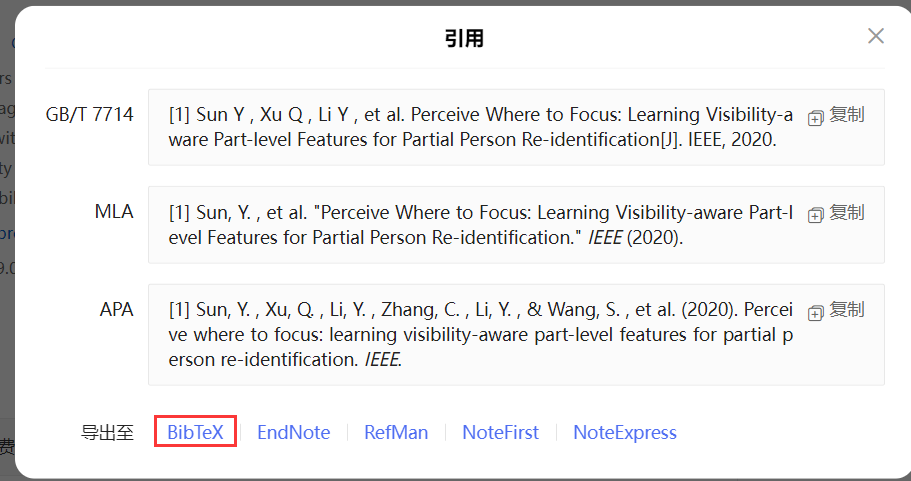
\includegraphics[height=4cm,width=10cm,trim=30 20 40 50,clip]{RefBaiduAcad}
	\caption{百度学术选择导出BibTex文件}
	\label{ref-baidu-academic}
\end{figure}

\begin{figure}[hp]
\centering
\subfigure[IEEE官网下载BibTeX文件]{
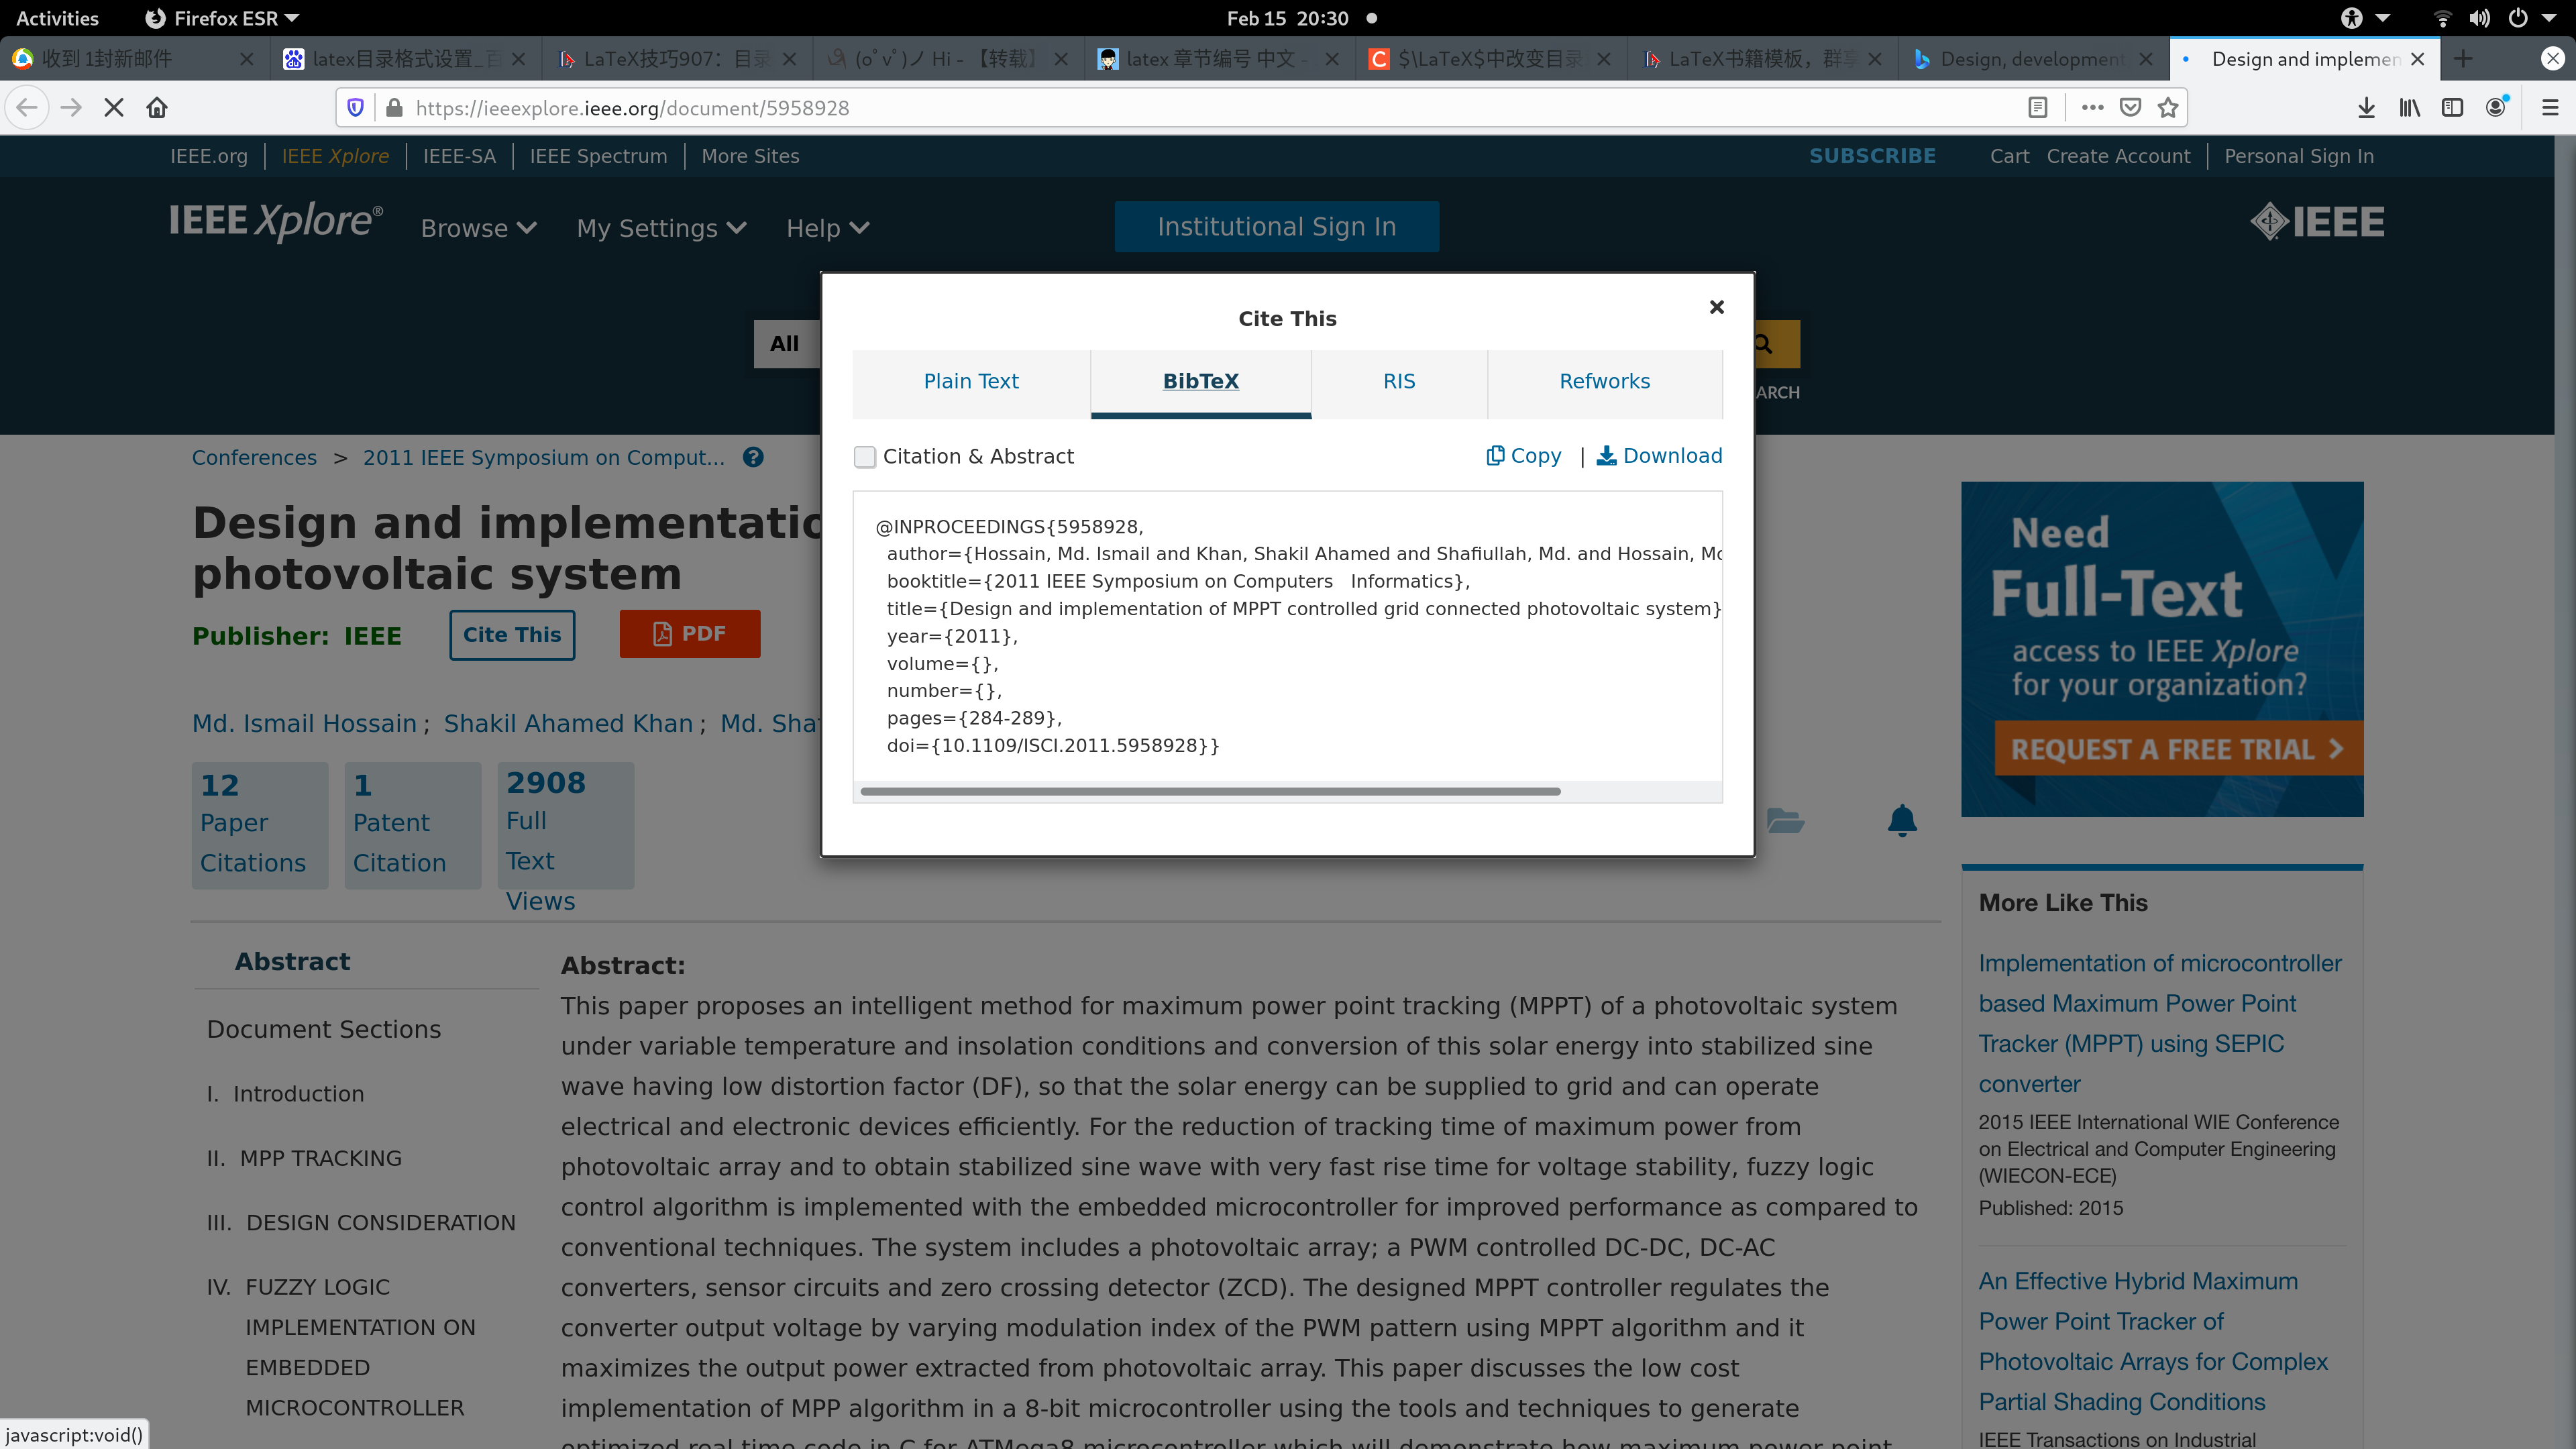
\includegraphics[width=8cm,trim=50 50 50 50,clip]{RefIEEE.png} \label{ref-ieee}
} 
\subfigure[Elsevier期刊官网选择导出BibTeX文件]{
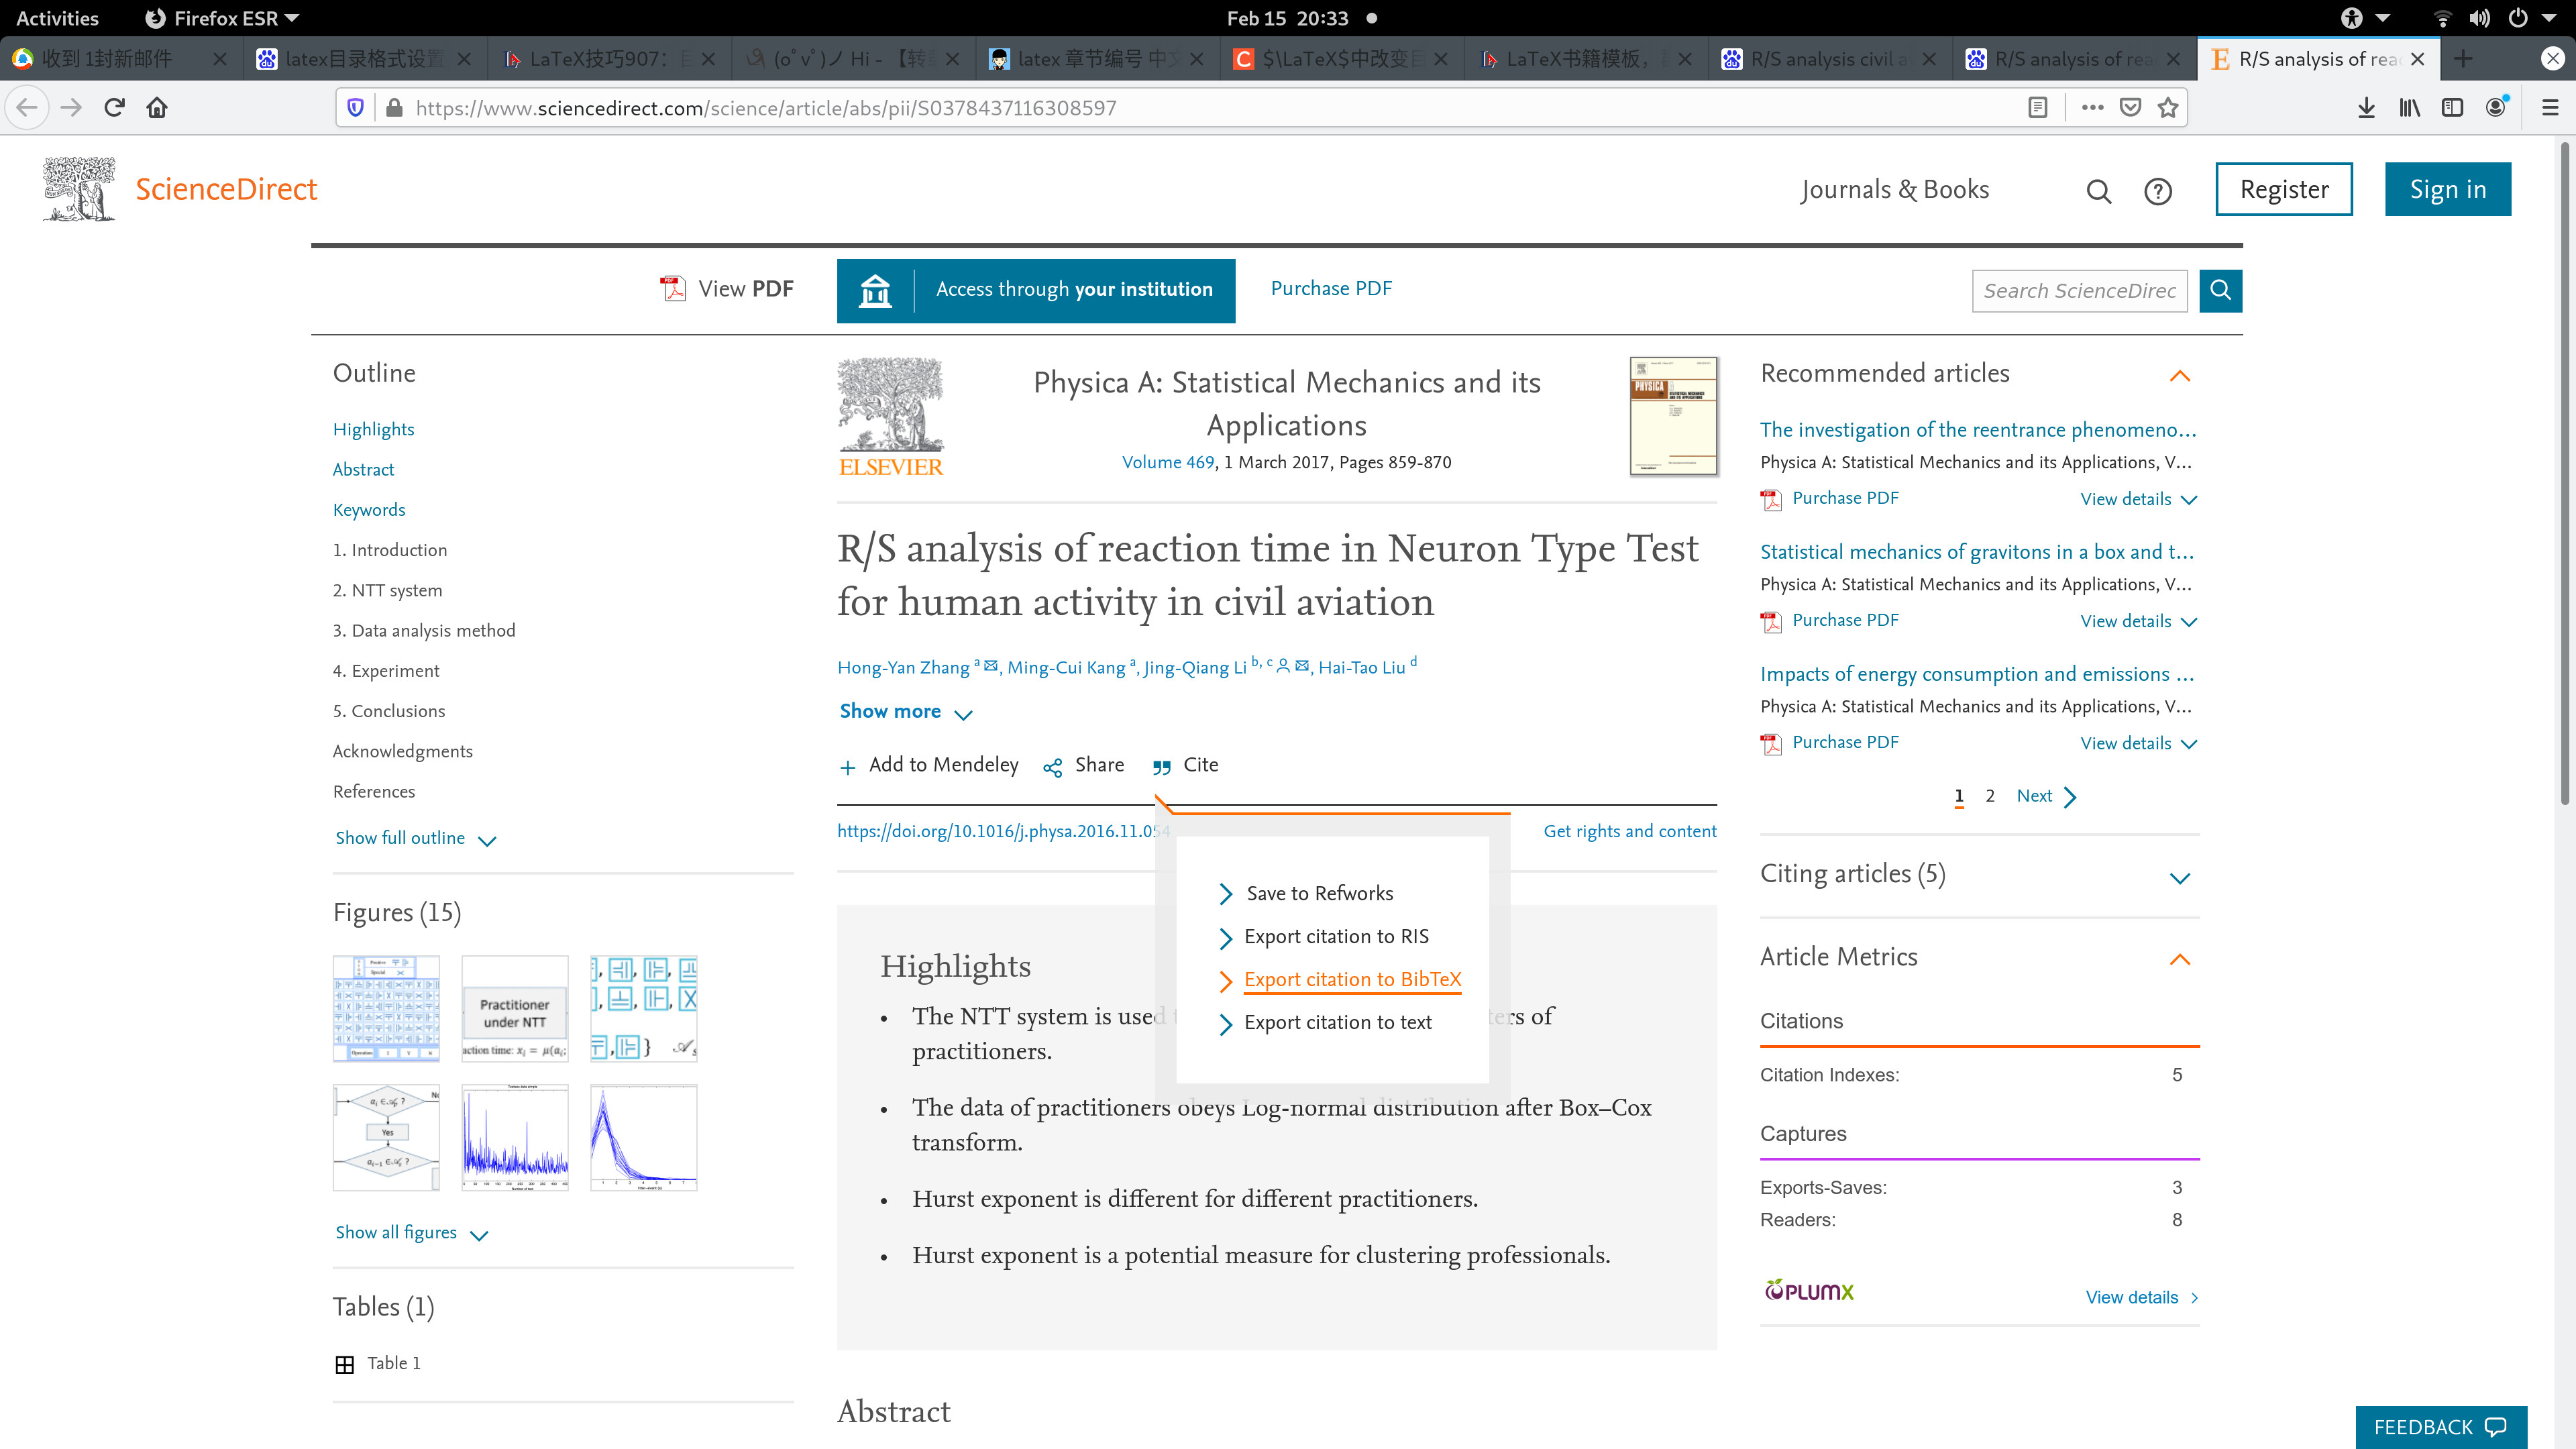
\includegraphics[width=8cm,trim=50 50 50 50,clip]{figures/RefElsevier.png} \label{ref-elsevier}
}
\caption{期刊网站上下载BibTeX文件: 信息通常不完整,需要自己补全}
\label{ref-infor-not-complete}
\end{figure}

\section{封面选择}

\subsection{本科生毕业设计或学位论文}
在\verb|main-BS.tex|文档中, 请在文档类型中进行设置。本科生授予的学位是学士,英文单词为
bachelor。
\begin{itemize}
\item 人文社科大类章节编号用中文,设置如下:\\
      \verb|\documentclass[chinesetitlenum,bachelor]{hainnuthesis}|
\item 理工科大类章节编号用数字,设置如下:\\
      \verb|\documentclass[arabictitlenum,bachelor]{hainnuthesis}|
\end{itemize}

\subsection{硕士与博士研究生学位论文}

\subsubsection{专业型学位论文与学术型学位论文}

专业型学位(例如电子信息专业硕士)与学术型学位(例如网络空间安全学术硕士)所采用的封面并不相同,你需要自己选择,这通过文档类型参数\verb|profesdegree|与\verb|academdegree|进行控制。
\begin{itemize}
\item 专业型学位,采用的设置如下:
	\begin{itemize}
	\item 理工大类请看profesdegree参数:\\
	  \verb|\documentclass[profesdegree,chinesetitlenum]{hainnuthesis}|
	\item 人文社科请看profesdegree参数:\\
	 \verb|\documentclass[profesdegree,arabictitlenum]{hainnuthesis}|
	\end{itemize} 
\item 学术型学位,采用的设置如下:
	\begin{itemize}
	\item 理工大类请看academdegree参数:\\
	 \verb|\documentclass[academdegree,chinesetitlenum]{hainnuthesis}|
	\item 人文社科请看academdegree参数:\\
	 \verb|\documentclass[academdegree,arabictitlenum]{hainnuthesis}|
	\end{itemize} 
\end{itemize}

\subsubsection{硕士论文与博士论文}
硕士与博士学位论文,在学位论文信息输入的参数设定列表中,利用\verb|degreelevel|
进行区分,如果是硕士则填写“硕士”,如果是博士则填写“博士” 


\section{章节编号差异与风格选择}

\subsection{理工科类专业章节编号}

理工科类专业文档的编号使用阿拉伯数字的方式居多,目录层级可能是: 
\begin{itemize}
\item 第~1~章
\item \quad 第~1~节
\item \qquad 第~1.1~小节
\end{itemize}
之类的风格。


\subsection{人文与社会科学类专业章节编号}

人文与社会科学类专业文档的编号使用汉字的方式居多,目录层级可能是: 
\begin{itemize}
\item 第一章
\item \quad 第一节
\item \qquad 第一小节
\end{itemize}
之类的风格, 或者是: 一、......;(一)、......;1、......之类的风格。

\subsection{章节编号与模板参数设定}

理工科与人文社科类专业有不同的章节编号传统,为了适应这个特点,在模板的文档类型中有一个参数项可以设定。在main.tex文档中的开头处,你可以找到相应的设定方法。
\begin{itemize}
\item 人文社科类编号, 可以按照如下方式设定:
     \begin{itemize}
     \item 专业型学位请看chinesetitlenum参数: \\
     \verb|\documentclass[profesdegree,chinesetitlenum]{hainnuthesis}|
     \item 学术型学位请看chinesetitlenum参数: \\
     \verb|\documentclass[academdegree,chinesetitlenum]{hainnuthesis}|
     \end{itemize}
\item 理工科科类编号, 可以按照如下方式设定:
     \begin{itemize}
     \item 专业型学位,请看arabictitlenum参数: \\
     \verb|\documentclass[arabictitlenum,profesdegree]{hainnuthesis}|
     \item 学术型学位,请看arabictitlenum参数:\\
      \verb|\documentclass[arabictitlenum,academdegree]{hainnuthesis}|
     \end{itemize}
\end{itemize}
这个采用参数arabictitlenum与chinesetitlenum控制章节编号风格的解决方案是由滴滴研
究院的工程师王子昊实现的,感谢他的帮助!

如果你对编号细节不满意,可以手动修改格式控制文件\verb|hainnuthesis.cls|中相应的地方,其它地方不要随意改动,免得发生错误自己难以控制。




\section{数学环境实例}

\subsection{行内公式与行间公式}

Newton第二定律,高中生喜欢写$f=ma$, 而大学生则经常写成$\displaystyle{f=m\fracode{v}{t}}$。定积分
$\displaystyle{\int^b_a g(x)\dif x}$可以用$G(b)-G(a)$来计算,其中$\displaystyle g(x) = \fracode{G(x)}{x}$。

你喜欢线性代数吗?我写个线性方程给你看看
\begin{equation}
\mat{A} \vec{x}= \vec{b}, \quad \mat{A}\in \ES{R}{n}{n}, \vec{x}\in \ES{R}{n}{1}
\end{equation}
特殊地,可以是
\begin{equation}
\mat{A} = \begin{bmatrix}
1 & 2 \\
2 & 3 
\end{bmatrix},\quad
\vec{x}=\begin{bmatrix}
x_1 \\ x_2
\end{bmatrix}, \quad
\vec{b} =\begin{bmatrix}
1 \\ 2
\end{bmatrix}
\end{equation}

\subsection{公式对齐}

这里有几个等式
\begin{equation}
\begin{split}
\int^b_a f(x)\dif x 
& = \int^b_a f(t)\dif t \\
& = \int^c_a f(x)\dif x + \int^b_c f(x)\dif x, \quad c\in [a,b] 
\end{split}
\end{equation}
还有别的等式
\begin{align}
\sum^n_{i=0} x^i 
&= 1 + x + \cdots + x^n \\
&= 1 + x(1 + x + \cdots + x^{n-1}) \\
& = 1 + x \sum^{n-1}_{j=0} x^j
\end{align}

概率公式: 对于$X\sim \mathcal{N}(\mu, \sigma^2)$, 可以得到
\begin{align}
\Prob(a \le X \le b) 
&=\Prob\left(\frac{a-\mu}{\sigma}\le \frac{X-\mu}{\sigma}\le
  \frac{b-\mu}{\sigma} \right) \\
&= \int^{\frac{b-\mu}{\sigma}}_{\frac{a-\mu}{\sigma}} \frac{1}{\sqrt{2\pi}}\me^{-x^2/2}\dif x \\
& = \Phi\left(\frac{b-\mu}{\sigma}\right) - \Phi\left(\frac{a-\mu}{\sigma}\right) 
\end{align}


\subsection{特殊环境}


这里有一个数学定义
\begin{definition}
对于函数$f: \Real \to \Real$, 如果它在点$x_0$处连续,那么它在该点处的导数规定为
\begin{equation}
f'(x_0) = \lim_{\Delta x\to 0} \frac{f(x_0 + \Delta x) - f(x_0)}{\Delta x}
\end{equation}
\end{definition}

\begin{definition}[内积]
$\ES{R}{n}{1}$上的内积规定为
\begin{equation}
\braket{\vec{a}}{\vec{b}} = \sum^n_{i=1} a_ib_i, \quad \forall \vec{a}, \vec{b}\in \ES{R}{n}{1}
\end{equation}
\end{definition}

写一个数学定理看看
\begin{theorem}
设直角三角形的直角边长分别为$a$与$b$, 斜边长为$c$, 那么
\begin{equation}
a^2 + b^2 = c^2
\end{equation}
\end{theorem}


写一个命题看看
\begin{proposition}
对于$\vec{a},\vec{b}\in \ES{R}{n}{1}$, Cauchy-Schwartz不等式成立
\begin{equation}
\abs{\braket{\vec{a}}{\vec{b}}}\le \norm{\vec{a}}\cdot \norm{\vec{b}}
\end{equation}
\end{proposition}



写一个例子看看

\begin{example}
定积分的可加性:
$$
\int^2_0 \sin \pi x \dif x = \int^1_0 \sin(\pi x) \dif x + \int^2_1 \sin(\pi x) \dif x
$$
\end{example}

\begin{example} 导数运算
\begin{align}
\fracode{[f(x)g(x)]}{x} 
&= f(x)\cdot \frac{g(x)}{x} + \fracode{f(x)}{x}\cdot g(x) \\
\fracpde{(uv)}{x}& = \fracpde{u}{x}v + u\fracpde{v}{x}\\
\nabla^2u(x,y,z)& = \lap{u}{x} + \lap{u}{y} +\lap{u}{z}
\end{align}
\end{example}

\begin{lemma} 如果对于任意的$f\in C[a,b]$, 等式
$$
\int^b_a g(x) f(x)\dif x = 0
$$
成立,那么$g(x)\equiv 0$.
\end{lemma}

\begin{property}[反对称性]
对于$\vec{a},\vec{b}\in \ES{R}{2}{1}$, 可以得到
$$
\det(\vec{a},\vec{b}) = - \det(\vec{b},\vec{a})
$$
\end{property}

\begin{property}[可加性]
对于$\vec{a},\vec{b},\vec{c}\in \ES{R}{2}{1}$, 可以得到
$$
\det(\vec{a}+\vec{b},\vec{c}) = \det(\vec{a},\vec{c}) +\det(\vec{b},\vec{c})
$$
\end{property}

\begin{property}[多重线性]
对于$\vec{a}_1,\vec{a}_2\in \ES{R}{2}{1}$以及$\lambda_1, \lambda_2\in\Real$, 可以得到
$$
\det(\lambda_1\vec{a}_1,\lambda_2\vec{a}_2) = \lambda_1\lambda_2 \det(\vec{a}_1,\vec{a}_2)
$$
\end{property}


\begin{corollary}
对于$\vec{a},\vec{b}\in \ES{R}{n}{1}$, 有
$$
\norm{\vec{a}+\vec{b}}^2 + \norm{\vec{a}-\vec{b}}^2 =2(\norm{\vec{a}}^2 +\norm{\vec{b}}^2)
$$
\end{corollary}



\section{流程图绘制}
\subsection{使用Tikz绘制流程图}
图~\ref{flowchart-tikz}是使用Tikz绘制的流程图。
\usetikzlibrary{shapes.geometric,arrows}
\usetikzlibrary{fit}
\usetikzlibrary{backgrounds}
\tikzstyle{startstop} = [rectangle, rounded corners, minimum width=3cm, minimum height=1cm, text centered, draw=black, fill=red!30]
\tikzstyle{io}        = [trapezium, trapezium left angle=70, trapezium right angle=110, minimum width=3cm, inner xsep = -15pt, minimum height=1cm, text centered, draw=black, fill=blue!30]
\tikzstyle{process}   = [rectangle, minimum width=3cm, minimum height=1cm, inner ysep=0, text centered, draw=black, fill=orange!30]
\tikzstyle{decision}  = [diamond,shape aspect=2.5, minimum width=3cm, minimum height=1cm, inner xsep=0,text centered, draw=black, fill=green!30]
\tikzstyle{arrow}     = [thick,->,>=stealth]

\begin{figure}[htp]
	\centering
	\begin{tikzpicture}[node distance=2cm]
		% adding nodes
		\node (start) [startstop] {Start};
		\node (io1)   [io, below of=start] {Lamp doesn't work};
		\node (dec1)  [decision, below of=io1] {Lamp plugged in?};
		\node (dec2)  [decision, below of=dec1, yshift=-0.3cm] {Bulb burned out?};
		
		\node (pro2) [process, below of=dec2] {Repair lamp};
		\node (stop) [startstop, below of=pro2] {Stop};
		
		\node (pro3) [process, left of=dec1, xshift=-2.5cm] {Plug in lamp};
		\node (pro4) [process, right of=dec2, xshift=2.5cm] {Replace bulb};
		
		% adding frame
		\begin{scope}[on background layer,label distance=1cm] % if you prefer pin, pin distance=1cm, and change label below to pin
			\node [draw=black!50,dashed,thick,fill=black!10,fit=(dec1) (dec2),label={[draw=red,fill=black!20,inner sep=0,anchor=south west]north east:{I am a node, too!}}] {};
		\end{scope}
		
		% adding arrows
		\draw [arrow] (start) -- (io1);
		\draw [arrow] (io1) -- (dec1);
		\draw [arrow] (dec1) -- node[anchor=east] {yes} (dec2);
		\draw [arrow] (dec2) -- node[anchor=east] {no } (pro2);
		
		\draw [arrow] (dec1) -- node[anchor=south] {no }(pro3);
		\draw [arrow] (dec2) -- node[anchor=south] {yes}(pro4);
		
		\draw [arrow] (pro4) |- (stop);
		\draw [arrow] (pro3) |- (stop);
		
		\draw [arrow] (pro2) -- (stop);
	\end{tikzpicture}
	\caption{使用Tikz绘制流程图}\label{flowchart-tikz}
\end{figure}

\subsection{插入其他软件绘制的流程图}
图~\ref{flowchart}~是使用Visio绘制后保存为jpg格式的流程图,使用正常插入图片的方法即可。
\begin{figure}[htp]			%需要图片在固定位置出现时,将h改为H
	\centering
	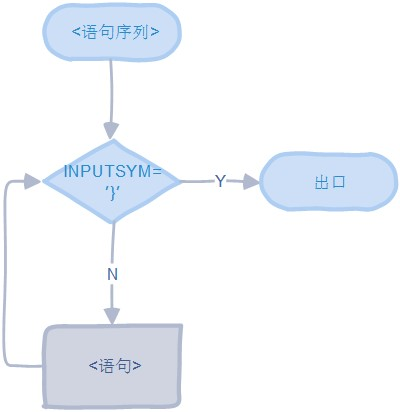
\includegraphics[width=6cm]{flowchart}
	\caption{使用Visio绘制的流程图} \label{flowchart}
\end{figure}

\subsection{Tikz绘制思维导图}
图~\ref{mindmap}是Tikz绘制的思维导图,关于Tikz更多信息可以查看\url{https://www.cnblogs.com/tsingke/p/6649800.html}
\begin{figure}[htp]
	\centering
	\begin{tikzpicture}[root concept/.append style = {concept color=blue,font = \color{white}\Large\bfseries },mindmap,scale=0.9]
		\tikzstyle{every node}=[font=\small,scale=0.9]
		\node[concept]{WebGIS}[clockwise from=0]
		child[grow=60,concept color = orange,font = \color{white}\bfseries \large ]{
			node[concept]{前端}		%这里是第二级节点
			[clockwise from  = 135]
			child[font = \color{white}\bfseries]{node[concept]{HTML}}
			child[font = \color{white}\bfseries]{node[concept]{CSS}}
			child[font = \color{white}\bfseries]{node[concept]{Vue}}
			child[font = \color{white}\bfseries]{node[concept]{Mapbox、Openlayers}}
		}
		child[grow=-60,concept color =   green!50!black,font=\color{white}\bfseries\kaishu\large]{
			node[concept]{后端} 
			[clockwise from = 45] 
			child[font = \color{white}\bfseries]{node[concept]{ArcGIS  API for Java}}
			child[font = \color{white}\bfseries]{node[concept]{ 高德 API }}
			child[font = \color{white}\bfseries]{node[concept]{Java Script}}
			child[font = \color{white}\bfseries]{node[concept]{源数据的获取-如Python爬虫}}
		};
	\end{tikzpicture}
	\caption{WebGIS 技术思维导图}\label{mindmap}
\end{figure}


\newpage

\section{表格示例}

\subsection{简单表格}

\begin{table}[htp]
	\caption{一个简单的表格}\label{tab1}
	\centering
	\begin{tabular}{|l|c|c|}
		\hline
		功能          &WEB         &APP         \\ \hline
		注册          &$\surd$     &$\surd$     \\ \hline
		登录          &$\surd$     &$\surd$     \\ \hline
		推送          &$\times$    &$\surd$     \\ \hline
	\end{tabular}
\end{table}

\begin{table}[htp]
	\caption{自定义表格}\label{tab2}
	\centering
	\begin{tabular*}{0.75\textwidth}{@{\extracolsep{\fill}}lcc}
		\toprule
		功能          &WEB         &APP         \\
		\midrule
		注册          &$\surd$     &$\surd$     \\
		登录          &$\surd$     &$\surd$     \\
		推送          &$\times$    &$\surd$     \\
		\bottomrule
	\end{tabular*}
\end{table}


\begin{table}[h]
\centering
\caption{绘制斜线表头}
\begin{tabular}{|c|c|c|c|c|c|c|}
\hline
\diagbox{节次}{\rotatebox{-45}{课程}}{星期} & 星期一 & 星期二 & 星期三 & 星期四 & 星期五 & 星期六 \\
\hline
上午 1-2 &  经济学  &  量子力学  &  微波原理 &  编译原理 & 计数组合学 & 学术讲座 \\  
\hline
上午 3-4 &  微波原理 & 学术写作  &  计数组合学& 经济学   & 民法典专题  & 学术讲座       \\ 
\hline 
\end{tabular}
\end{table}

\subsection{复杂表格}

去网站\url{https://www.tablesgenerator.com/latex_tables}看看,你肯定会喜欢的!更改好表格的数据后,点击Generate即可生成\LaTeX 代码!

\subsection{支持自动添加表头的换页表格}
如表~\ref{tab4}~所示.
\begin{center}
	\begin{longtable}{cp{1.5cm}cp{2cm}}
		\caption{某个用于测试的表格} \label{tab4} \\
		\hline
		\textbf{$x$}& \textbf{$sinx$} & \textbf{$5x^{2}+3x+3$}& \textbf{$log_{10}x$}\\
		\hline
		\endfirsthead
		\caption*{某个用于测试的表格(续)}\\
		\hline
		\textbf{$x$}& \textbf{$sinx$} & \textbf{$5x^{2}+3x+3$}& \textbf{$log_{10}x$}\\
		\hline
		\endhead
		\hline
		\endfoot
		\hline
		\endlastfoot
		1.00 & 0.02 & 11.00 & 0.00\\
		2.00 & 0.03 & 29.00 & 0.30\\
		3.00 & 0.05 & 57.00 & 0.48\\
		4.00 & 0.07 & 95.00 & 0.60\\
		5.00 & 0.09 & 143.00 & 0.70\\
		6.00 & 0.10 & 201.00 & 0.78\\
		7.00 & 0.12 & 269.00 & 0.85\\
		8.00 & 0.14 & 347.00 & 0.90\\
		9.00 & 0.16 & 435.00 & 0.95\\
		10.00 & 0.17 & 533.00 & 1.00\\
		11.00 & 0.19 & 641.00 & 1.04\\
		12.00 & 0.21 & 759.00 & 1.08\\
		13.00 & 0.22 & 887.00 & 1.11\\
		14.00 & 0.24 & 1025.00 & 1.15\\
		15.00 & 0.26 & 1173.00 & 1.18\\
		16.00 & 0.28 & 1331.00 & 1.20\\
		17.00 & 0.29 & 1499.00 & 1.23\\
		18.00 & 0.31 & 1677.00 & 1.26\\
		19.00 & 0.33 & 1865.00 & 1.28\\
		20.00 & 0.34 & 2063.00 & 1.30\\
		21.00 & 0.36 & 2271.00 & 1.32\\
		\hline
	\end{longtable}
\end{center}
这种形式比较好,续表可以带上表头,阅读方便,看起来美观。

\subsection{另一种跨页表格}
表~\ref{tab5}~是另一种跨页表格,只不过没法在每一页都生成caption。

\tablehead{\hline $x$ & $sinx$ & $5x^{2}+3x+3$ & $log_{10}x$ \\ \hline}
\tablecaption{另一种跨页表格}
\tabletail{\hline}
\begin{center}
	
\label{tab5}
	\begin{supertabular}{cccc}
		\hline
		1.00 & 0.02 & 11.00 & 0.00\\
		2.00 & 0.03 & 29.00 & 0.30\\
		3.00 & 0.05 & 57.00 & 0.48\\
		4.00 & 0.07 & 95.00 & 0.60\\
		5.00 & 0.09 & 143.00 & 0.70\\
		6.00 & 0.10 & 201.00 & 0.78\\
		7.00 & 0.12 & 269.00 & 0.85\\
		8.00 & 0.14 & 347.00 & 0.90\\
		9.00 & 0.16 & 435.00 & 0.95\\
		10.00 & 0.17 & 533.00 & 1.00\\
		11.00 & 0.19 & 641.00 & 1.04\\
		12.00 & 0.21 & 759.00 & 1.08\\
		13.00 & 0.22 & 887.00 & 1.11\\
		14.00 & 0.24 & 1025.00 & 1.15\\
		15.00 & 0.26 & 1173.00 & 1.18\\
		16.00 & 0.28 & 1331.00 & 1.20\\
		17.00 & 0.29 & 1499.00 & 1.23\\
		18.00 & 0.31 & 1677.00 & 1.26\\
		19.00 & 0.33 & 1865.00 & 1.28\\
		20.00 & 0.34 & 2063.00 & 1.30\\
		21.00 & 0.36 & 2271.00 & 1.32\\
		\hline
	\end{supertabular}
\end{center}

\subsection{表格横置}

有时候表格太宽了,需要横向放置,可以采用\verb|\usepackage{lscape}|并配合命令
\begin{verbatim}
	\begin{landscape}
		% your table here
	\end{landscape}
\end{verbatim}
进行设定。需要注意的是,横置了就会占用至少一页的空间。一个小例子如下所示。
	\begin{landscape}
	\begin{table}
		\centering
		\caption{一个横着放的小表格}
		\begin{tabular}{cccp{2cm}p{2cm}}
			\hline
			Aqqq & Bqqq & Cqqq & Dqqq & Eqqqqq \\
			\hline
			1 & 2 & 3 & 4 & 5\\
			A & B & C & D & E \\
			1 & 2 & 3 & 4 & 5\\
			A & B & C & D & E \\
			1 & 2 & 3 & 4 & 5\\
			A & B & C & D & E \\
			1 & 2 & 3 & 4 & 5\\
			A & B & C & D & E \\
			1 & 2 & 3 & 4 & 5\\
			\hline
		\end{tabular}
	\end{table}
\end{landscape}
\subsection{表格跨页同时也横置}
这里有一个长表格,也横置了,很占地方呀!
\begin{landscape}
		\begin{longtable}{cm{4cm}ccp{4cm}c}
		\caption{某个用于测试的表格} \label{tab4} \\
		\hline
		$x$ & $sinx$ & $cosx$ & $5x^{2}+3x+3$ & $log_{10}x$ & $3x+5$\\
		\hline
		\endfirsthead
		\caption*{某个用于测试的表格(续)}\\
		\hline
		$x$ & $sinx$ & $cosx$ & $5x^{2}+3x+3$ & $log_{10}x$ & $3x+5$\\
		\hline
		\endhead
		\hline
		\endfoot
		\hline
		\endlastfoot
		1.00 & 0.02 & 1.00 & 11.00 & 0.00 & 8.00\\
		2.00 & 0.03 & 1.00 & 29.00 & 0.30 & 11.00\\
		3.00 & 0.05 & 1.00 & 57.00 & 0.48 & 14.00\\
		4.00 & 0.07 & 1.00 & 95.00 & 0.60 & 17.00\\
		5.00 & 0.09 & 1.00 & 143.00 & 0.70 & 20.00\\
		6.00 & 0.10 & 0.99 & 201.00 & 0.78 & 23.00\\
		7.00 & 0.12 & 0.99 & 269.00 & 0.85 & 26.00\\
		8.00 & 0.14 & 0.99 & 347.00 & 0.90 & 29.00\\
		9.00 & 0.16 & 0.99 & 435.00 & 0.95 & 32.00\\
		10.00 & 0.17 & 0.98 & 533.00 & 1.00 & 35.00\\
		11.00 & 0.19 & 0.98 & 641.00 & 1.04 & 38.00\\
		12.00 & 0.21 & 0.98 & 759.00 & 1.08 & 41.00\\
		13.00 & 0.22 & 0.97 & 887.00 & 1.11 & 44.00\\
		14.00 & 0.24 & 0.97 & 1025.00 & 1.15 & 47.00\\
		15.00 & 0.26 & 0.97 & 1173.00 & 1.18 & 50.00\\
		16.00 & 0.28 & 0.96 & 1331.00 & 1.20 & 53.00\\
		17.00 & 0.29 & 0.96 & 1499.00 & 1.23 & 56.00\\
		18.00 & 0.31 & 0.95 & 1677.00 & 1.26 & 59.00\\
		19.00 & 0.33 & 0.95 & 1865.00 & 1.28 & 62.00\\
		20.00 & 0.34 & 0.94 & 2063.00 & 1.30 & 65.00\\
		21.00 & 0.36 & 0.93 & 2271.00 & 1.32 & 68.00\\
		22.00 & 0.37 & 0.93 & 2489.00 & 1.34 & 71.00\\
		23.00 & 0.39 & 0.92 & 2717.00 & 1.36 & 74.00\\
		24.00 & 0.41 & 0.91 & 2955.00 & 1.38 & 77.00\\
		25.00 & 0.42 & 0.91 & 3203.00 & 1.40 & 80.00\\
		26.00 & 0.44 & 0.90 & 3461.00 & 1.41 & 83.00\\
		27.00 & 0.45 & 0.89 & 3729.00 & 1.43 & 86.00\\
		28.00 & 0.47 & 0.88 & 4007.00 & 1.45 & 89.00\\
		29.00 & 0.48 & 0.87 & 4295.00 & 1.46 & 92.00\\
		30.00 & 0.50 & 0.87 & 4593.00 & 1.48 & 95.00\\
		31.00 & 0.52 & 0.86 & 4901.00 & 1.49 & 98.00\\
		32.00 & 0.53 & 0.85 & 5219.00 & 1.51 & 101.00\\
		33.00 & 0.54 & 0.84 & 5547.00 & 1.52 & 104.00\\
		34.00 & 0.56 & 0.83 & 5885.00 & 1.53 & 107.00\\
		35.00 & 0.57 & 0.82 & 6233.00 & 1.54 & 110.00\\
		36.00 & 0.59 & 0.81 & 6591.00 & 1.56 & 113.00\\
		\hline
	\end{longtable}
\end{landscape}
\newpage 

\section{程序代码示例}

\subsection{代码片段}
这里有几行C程序代码, 虽然没加方框,但是添加了行号。
\begin{lstlisting}[language=C]
	typedef double (*Ptr2Fun)(double); /*创建新数据类型: 函数指针*/
	Ptr2Fun f; /* 声明函数指针类型的变量  */
	f = cos;   /* 给变量赋值 */
	Ptr2Fun g = sin; /* 定义函数指针型变量, 存在内存分配的动作 */
	const double pi = acos(-1.0); //  定义常数 pi = 3.1415926... 
	double value_1 = g(pi/2); // value_1 = sin(pi/2) = 1.0  
	double value_2 = g(pi/4); // value_2 = sin(pi/4) = 0.707 ... 
\end{lstlisting}

\subsection{完整的小程序}
采用``分割---近似---求和"的方法计算定积分的数值
$$
\int^b_a f(x) \mathrm{d} x \approx \sum^{n-1}_{i=0} f(x_i)\Delta x, \quad x_i = a+i\cdot \Delta x, \quad \Delta x = \frac{b-a}{n}
$$
\begin{lstlisting}[language=C,frame=shadowbox,title={Integral-1.c}]
	double Integral(Ptr2Fun f, double a, double b, unsigned n)
	{
		double sum = 0.0, delta_x = (b-a)/n;
		double x_i = 0.0;
		for(int i = 0; i < n; i++){
			x_i = a + i*delta_x;
			sum += f(x_i)*delta_x;
		}
		return sum; 				
	}
\end{lstlisting}

\subsection{将整个源代码文件导入\LaTeX{}文档中}
你可以使用\verb*|\lstinputlisting{}|命令将程序的源代码导入\LaTeX 文档,这样就免除了复制操作可能带来的错误。

\textbf{\textcolor[rgb]{0.98,0,0}{Input Python source:}}
\lstinputlisting[language=Python,frame=shadowbox]{code/example.py}

\subsection{使用{\LaTeX{}}命令给代码写注释}

\begin{lstlisting}[language=C,frame=shadowbox,title={Integral-2.c}]
    /* 计算定积分 (*@$\displaystyle \int^b_a f(x)\mathrm{d} x \approx \sum^{n-1}_{i=0} f(x_i)\Delta x_i $@*) */
	double Integral(Ptr2Fun f, double a, double b, unsigned n)
	{
		double sum = 0.0, delta_x = (b-a)/n; 
		double x_i = 0.0;
		for(int i = 0; i < n; i++){
			x_i = a + i*delta_x;   /* (*@$ x_i = a + i\cdot \Delta x $@*) */
			sum += f(x_i)*delta_x; /* (*@$ S \leftarrow S + f(x_i)\cdot \Delta x $@*) */
		}
		return sum; 				
	}
\end{lstlisting}


\subsection{算法与伪代码示例}

算法~\ref{alg-1}~对于xxx来说是关键,其显著的特点是xxx, 

\begin{algorithm}[h]
	\caption{如何使用while和if} \label{alg-1}
	\begin{algorithmic}[1]  %每行显示行号
		\Require 这段代码
		\Ensure 使用while和if的方法
		\Function{函数名}{参数列表}
		\While{True}
		\If{临界条件}
		\State 退出循环
		\EndIf
		\State 某个变量  $\gets$ 某个变量
		\EndWhile
		\State\Return 某个返回值
		\EndFunction
	\end{algorithmic}
\end{algorithm}

算法~\ref{alg-2}~对于xxx来说是关键,其显著的特点是xxx, 

\begin{breakablealgorithm}
	\caption{如何使用for和do-while} \label{alg-2}
	\begin{algorithmic}[1]  %每行显示行号
		\Require 这段代码
		\Ensure 使用for和do-while的方法
		\Function{函数名}{参数列表}
		\Repeat
		\State 学习\LaTeX
		\Until{Alive}
		\For{$ i = 1, 2, ..., 7 $}
		\State echo "今天是周\$i\ "
		\EndFor
		\EndFunction
	\end{algorithmic}
\end{breakablealgorithm}


\section{参考文献使用示例}

对于论文的写作而言,文献的引用无疑是非常重要的。言之有理,言之有据,这是基本的要求。文献引用,需要使用命令\verb|\cite|与文献条码标签。在中国大陆地区,有参考文献的国家标准,即GB/T 7714, 请你注意这个标准。本模板采用的参考文献格式复合这个标准,是自动利用BibTeX文件自动生成的, 这得感谢开发gbt7714宏包的作者与维护者们! 这里有几种不同类型的参考文献:

\begin{itemize}
\item[\ding{172}] 期刊论文, 例如\cite{XmDeng2007,Brown1984,ZHY2017RS,ZHY2012manifold}以及\cite{Wing2006CT}
\item[\ding{173}] 会议论文, 例如\cite{Geyer1999,Branislav2004}
\item[\ding{174}] 专利, 例如\cite{LongMA2015P}
\item[\ding{175}] 书籍, 例如\cite{CDIO2014,ZHY2022}
\item[\ding{176}] 在线资源, 例如\cite{SFMedu,OpenMVS,HainnuThesis}
\item[\ding{177}] 技术报告,例如\cite{Sussman2005}
\item[\ding{178}] 学位论文,例如\cite{ZHY2002,Xue2006,lzj-zhy-MS-thesis-2018,zls-zhy-MS-thesis-2016,zhy-2011-disertation}


脚注一\footnote{康宁. 中国发展研究基金会丛书:《和谐社会的治理之道――领导者的讲述》[M].},
脚注二\footnote{康宁. 中国发展研究基金会丛书:《和谐社会的治理之道――领导者的讲述》[M].}。
脚注三\footnote{康宁. 中国发展研究基金会丛书:《和谐社会的治理之道――领导者的讲述》[M].}。

引用参考文献一\cite{gao1987},引用参考文献二\cite{zhang1989}。

引用参考文献一和二\cite{gao1987,zhang1989}。


\end{itemize}



%%==================================%%
%%            结     论            %%
%%==================================%%
%%==================================%%
%%            结 论 章              %%
%%==================================%%
\conclusion


我的结论是什么我的结论是什么我的结论是什么我的结论是什么我的结论是什么我的结论
是什么我的结论是什么我的结论是什么我的结论是什么我的结论是什么我的结论是什么我
的结论是什么我的结论是什么. 我的结论是什么我的结论是什么我的结论是什么我的结论
是什么我的结论是什么我的结论是什么我的结论是什么我的结论是什么我的结论是什么我的
结论是什么我的结论是什么我的结论是什么. 我的结论是什么我的结论是什么我的结论是什
么我的结论是什么我的结论是什么我的结论是什么我的结论是什么我的结论是什么我的结论
是什么我的结论是什么我的结论是什么

我的结论是什么我的结论是什么我的结论是什么我的结论是什么我的结论是什么我的结论
是什么我的结论是什么我的结论是什么我的结论是什么我的结论是什么我的结论是什么我
的结论是什么我的结论是什么. 我的结论是什么我的结论是什么我的结论是什么我的结论
是什么我的结论是什么我的结论是什么我的结论是什么我的结论是什么我的结论是什么我的
结论是什么我的结论是什么我的结论是什么. 我的结论是什么我的结论是什么我的结论是什
么我的结论是什么我的结论是什么我的结论是什么我的结论是什么我的结论是什么我的结论
是什么我的结论是什么我的结论是什么

我的结论是什么我的结论是什么我的结论是什么我的结论是什么我的结论是什么我的结论
是什么我的结论是什么我的结论是什么我的结论是什么我的结论是什么我的结论是什么我
的结论是什么我的结论是什么. 我的结论是什么我的结论是什么我的结论是什么我的结论
是什么我的结论是什么我的结论是什么我的结论是什么我的结论是什么我的结论是什么我的
结论是什么我的结论是什么我的结论是什么. 我的结论是什么我的结论是什么我的结论是什
么我的结论是什么我的结论是什么我的结论是什么我的结论是什么我的结论是什么我的结论
是什么我的结论是什么我的结论是什么



%%==================================%%
%%             附    录             %%
%%==================================%%
\appendices
\section{数学预备知识}
\subsection{线性代数}
你喜欢线性代数吗?我写个线性方程给你看看
\begin{equation}
	\mat{A} \vec{x}= \vec{b}, \quad \mat{A}\in \ES{R}{n}{n}, \vec{x}\in \ES{R}{n}{1}
\end{equation}
特殊地,可以是
\begin{equation}
	\mat{A} = \begin{bmatrix}
		1 & 2 \\
		2 & 3 
	\end{bmatrix},\quad
	\vec{x}=\begin{bmatrix}
		x_1 \\ x_2
	\end{bmatrix}, \quad
	\vec{b} =\begin{bmatrix}
		1 \\ 2
	\end{bmatrix}
\end{equation}

图~\ref{hnulogo}是海师logo图片, 代码中有裁剪图片的参数设定细节。
\begin{figure}[hp]
	\centering
	
\includegraphics[height=4cm,width=10cm,trim=30 20 40 50,clip]{logo}
	\caption{裁剪海师logo图片,裁剪尺寸参数的顺序依次是“左-下-右-上”}
	\label{hnulogo}
\end{figure}

\begin{table}[htp]
	\caption{一个简单的表格}\label{tab1}
	\centering
	\begin{tabular}{|l|c|c|}
		\hline
		功能          &WEB         &APP         \\ \hline
		注册          &$\surd$     &$\surd$     \\ \hline
		登录          &$\surd$     &$\surd$     \\ \hline
		推送          &$\times$    &$\surd$     \\ \hline
	\end{tabular}
\end{table}

\subsection{微积分}
Newton第二定律,高中生喜欢写$f=ma$, 而大学生则经常写成$\displaystyle{f=m\fracode{v}{t}}$。定积分
$\displaystyle{\int^b_a g(x)\dif x}$可以用$G(b)-G(a)$来计算,其中$\displaystyle g(x) = \fracode{G(x)}{x}$。

这里有几个等式
\begin{equation}
	\begin{split}
		\int^b_a f(x)\dif x 
		& = \int^b_a f(t)\dif t \\
		& = \int^c_a f(x)\dif x + \int^b_c f(x)\dif x, \quad c\in [a,b] 
	\end{split}
\end{equation}
%\zhlipsum[1-3]

\section{下载文献}

\subsection{电子书}

学位论文的写作经常需要选择阅读参考文献,书籍是总会遇到的. 这里有个网站可以下载电子书,免费的,你可以试试打开这个网页链接: \url{https://blog.passernav.com/411.html}, 网页上会列出你可以选择能用的可访问地址列表,正常情况下每天都会更新! 

\subsection{论文}

各个高校的图书馆中可以下载一些电子版的论文,包括期刊与会议论文。还有个大名鼎鼎的SCI-HUB网站,你不要错过, 其官网是: \url{https://www.scihub.net.cn/}.
找不到的时候,找找你的老同学,在不同大学或研究机构的,找他们帮忙,或者给论文的作者发邮件请求她或他给你发一份拜读一下。记得态度要诚恳要好!

还有一些Preprint版本的论文网站,例如大名鼎鼎的~\url{https://arxiv.org}, 可以去看看。


%%****************************************
%%  参考文献
%%****************************************
% 按照国家标准生成参考文献,采用数字编号进行排序
\bibliographystyle{gbt7714-numerical}
\reference\nointerlineskip
\bibliography{BibTeX/BibTest}

%%==================================%%
%%             学术成果             %%
%%==================================%%
\achievements

\noindent
一、公开发表的论文及著作
\begin{table}[hbp]
    \zihao{-4}\linespread{1.1}\selectfont
    \renewcommand\arraystretch{1.2}
    \setlength\tabcolsep{6pt}
    \begin{tabular}{|C{.375\textwidth}|C{.175\textwidth}|C{.14\textwidth}|C{.09\textwidth}|C{.0715\textwidth}|}
        \hline
        \textbf{文章名称} & \textbf{发表刊物(出版社)} & \textbf{刊发时间与卷期号} & \textbf{刊物级别} & \textbf{第几作者} \\ \hline
        X X X X X X X X & 《X X X X X X》 & 2003年第1期 & CSSCI & 1 \\ \hline
        X X X X X X X X X X X X X X X & 《X X X X X》 & 2002年第9期 & 核心期刊 & 2 \\ \hline
        X X X X X X X X X X X X X X X & 《X X X X X X X》 & 2002年第10期 & 核心期刊 & 1 \\ \hline
        X X X X X X X X & 《X X X X X X》 & 2003年第1期 & 核心期刊 & 1 \\ \hline
        X X X X X X X & 教育科学出版社 & 2004年12月 &  & 1 \\ \hline
    \end{tabular}
\end{table}

\noindent
二、相关的其它成果(包括专利、获奖项目等)

%%==================================%%
%%             致    谢             %%
%%==================================%%
\acknowledgement


\zhlipsum[1-3]

%%==================================%%
%%             答辩决议             %%
%%==================================%%
%\resolution

答辩决议答辩决议


\end{document}
